\documentclass[landscape,twocolumn,a4paper]{article}
\usepackage[utf8x]{inputenc}
\usepackage[ngerman]{babel}
\usepackage{listings}
\usepackage{babel}

\usepackage[T1]{fontenc}
\usepackage{booktabs} % schöne Tabellen
\usepackage{graphicx}
\usepackage{csquotes} % Anführungszeichen
\usepackage{paralist} % kompakte Aufzählungen
\usepackage{amsmath,textcomp,tikz} %diverses
\usepackage{eso-pic} % Bilder im Hintergrund
\usepackage{mdframed} % Boxen
\usepackage{multirow}
\usepackage{amssymb}

\usepackage{mathtools}
\usepackage[top=20mm,left=10mm,right=10mm,bottom=10mm]{geometry}
\usepackage{fancyhdr}
\pagestyle{fancy}
\fancyhead[L]{Aufgaben zu Zahlentheorie/Kryptographie}
\fancyhead[R]{\thepage}
\fancyfoot{}

\lstset{language=Python, tabsize=4, basicstyle=\footnotesize, showstringspaces=false, mathescape=true}
\lstset{literate=%
  {Ö}{{\"O}}1
  {Ä}{{\"A}}1
  {Ü}{{\"U}}1
  {ß}{{\ss}}1
  {ü}{{\"u}}1
  {ä}{{\"a}}1
  {ö}{{\"o}}1
}
\begin{document}
\newcommand{\ggT}{\operatorname{ggT}}
\newcommand{\Mod}[3]{#1\equiv#2\mod#3}
\newcommand\x{1}
\newcounter{y}
\setcounter {y} {1}

\parindent 0mm



\textbf{Diophantische Gleichungen} 
\bigskip

\textbf{A1a:}   \\
Zerlege die Zahlen in Primfaktoren und bestimme damit den ggT. Bestimme dann nochmal den ggT mit
dem Euklidschen Algorithmus. \\
a.  $a = 315, b=693$ \quad b. $a=336,b=264$
\bigskip  

\textbf{A\arabic {y}:}   \\
Berechne mit dem Euklidischen Algorithmus: \\
a.  $\ggT(150,54)$ \quad b. $\ggT(300,468)$ \quad 
 c.$\ggT(44,18)$ \quad d. $\ggT(992,999)$
\bigskip \stepcounter{y}
 
\textbf{A\arabic {y}:}   \\
Berechne den ggT der Zahlen $a$ und $b$ und stelle ihn in der Form $ax + by$ dar. \\
a.   $ a = 531, b = 93$  \quad b. $ a = 753, b = 64$
\bigskip \stepcounter{y}

\textbf{A\arabic {y}:}   \\
Bestimme - falls möglich - eine Lösung $(x/y)$ der angegebenen Gleichung: \\
a.  $96x+66y=6$ \quad b.$96x+66y=18$ \\
d.  $119x+143y=4$ \quad e. $91x+35y=12$.
\bigskip \stepcounter{y}
 
 
 \textbf{A\arabic {y}:}   \\
Vereinfache die Gleichung und finde möglichst viele Lösungen: \\
a.   $42x+126y=84$ \quad b. $81x+54y=27$ \quad 
 c. $77x+121y=44$ 
 \bigskip \stepcounter{y}

 
 \textbf{Kongruenzen} \bigskip
 
\textbf{A\arabic {y}:}   \\
Bestimme möglichst alle ganzzahligen Lösungen $x$ der folgenden
  Gleichungen: \\
a. $\Mod{5+x}{2}{7}$\quad b.   $\Mod{5\cdot x}{2}{7}$ \\ 
c. $\Mod{5\cdot x}{2}{10}$  \quad d.  $\Mod{-34}{x}{5}$
\bigskip \stepcounter{y}

\textbf{A\arabic {y}:}   \\
Beweise die folgenden Aussagen:\\
a. Wenn $\Mod{a}{b}{m}$ und $\Mod{c}{d}{m}$, dann
    $\Mod{a+c}{b+d}{m}$. \\
b. Wenn $\Mod{a}{b}{m}$, dann $\Mod{-a}{-b}{m}$. \\
c. Wenn $\Mod{a}{b}{m}$ und $\Mod{b}{c}{m}$, dann
    $\Mod{a}{c}{m}$.
\bigskip \stepcounter{y}

 \textbf{Restklassen} \bigskip

\textbf{A\arabic {y}:}   \\
Bestimme mit dem erweiterten Euklidschen Algorithmus: \\
 a.  $\dfrac{\overline{5}}{\overline{33}}$ in  $\mathbb{Z}_{37}$. \quad
 b.  $\dfrac{\overline{7}}{\overline{20}}$ in  $\mathbb{Z}_{89}$.
\bigskip \stepcounter{y}

\textbf{A\arabic {y}:}   \\
Bestimme mit dem kleinen Satz von Fermat: \\
 a.  $\overline{4}^{-11}$ in  $\mathbb{Z}_{13}$. \quad
 b.  $\overline{6}^{31}$ in  $\mathbb{Z}_{29}$. \quad
 c.  $ \overline{6}^{32}$ in  $\mathbb{Z}_{29}$. 
\bigskip \stepcounter{y}

\textbf{A\arabic {y}:}   \\
Berechne in $\mathbb{Z}_{23}$ die folgenden Brüche: \\
a.  $\dfrac{\overline{1}}{\overline{5}^{21}} $ \quad
b.  $\dfrac{\overline{1}}{\overline{10}^{13}} $ \quad
c.  $\dfrac{\overline{7}}{\overline{10}^{12}} $ \quad
d.  $\dfrac{\overline{7}}{\overline{22}} $ 

\bigskip
Prüfe, ob die angegebene Zahl eine Primitivwurzel ist: \\
 e. 4 in  $\mathbb{Z}_{13}$ \quad  f. 6 in  $\mathbb{Z}_{13}$
\bigskip \stepcounter{y}

\textbf{Diffie-Hellman} \bigskip

\textbf{A\arabic {y}:}   \\
a. Alice und Bob vereinbaren die Primzahl p und die Primitivwurzel g.
Alice wählt a, Bob wählt b. Welche Zahlen werden veröffentlicht und wie heißt der gemeinsame Schlüssel?

a.  p = 7, g = 3, a = 3, b = 4.  \quad
b.  p = 23, g = 7, a = 15, b = 17.

\bigskip \stepcounter{y}

\textbf{A\arabic {y}:}   \\
Alice und Bob vereinbaren p = 11 und g = 2. Alice schicht an Bob A = 5 und Bob meldet an Alice B = 8. Da die Zahlen klein sind, kann die Diffie-Hellman Verschlüsselung geknackt werden.  Wie heißt der Schlüssel K?

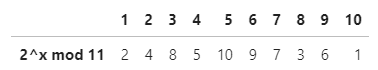
\includegraphics[width=6.9cm]{potenzen.png}
\bigskip \stepcounter{y}

\textbf{RSA} \bigskip

\textbf{A\arabic {y}:}   \\
Bob wählt p , q  und Verschlüsselungsexponent e. Warum ist e ein
zulässiger Verschlüsselungsexponent? Wie heißt der öffentliche, wie der private Schlüssel von Bob?
Alice will an Bob die Nachricht n verschlüsselt übermitteln.  
Welche Zahl schickt sie an Bob? Wie entschlüsselt Bob die Nachricht?

a.  p = 3, q = 11,  e = 7, n = 6. \quad
b.  p = 7, q = 11, e = 47, n = 2 

\newpage

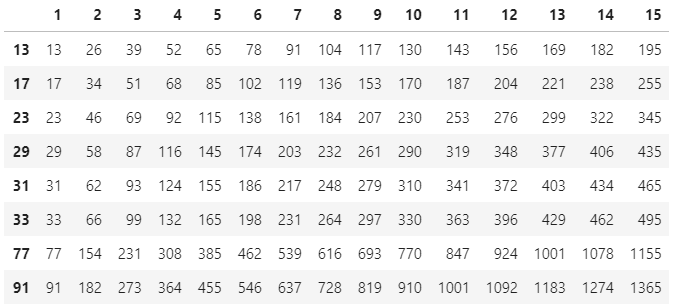
\includegraphics[width=12cm]{reihen.png}

Quadratzahlen: \\
11-121 12-144 13-169 14-196 15-225 16-256 17-289 18-324 19-361 20-400 
21-441 22-484 23-529 24-576 25-625 26-676 27-729 28-784 29-841 30-900 


\bigskip \stepcounter{y}
\bigskip \stepcounter{y}
\end{document}
